\section{Features explanation}
    In this thesis, the system must have the ability to control devices in the house in a convenient way, which means user can control devices from anywhere, anytime they want with an Internet-connected device and timer. Furthermore, the house should be capable of providing scenarios depends on the needs of user. For instance, users can switch on or off a number of specific devices by choosing a scenario instead of choosing individual device, namely “I’m home”, “Good night”, or “I’m leaving”. Based on the basic ideas, the thesis is integrated with all the basic features above. The thesis is designed for an one-floor house with three rooms, namely Living Room, Dining Room and Bedroom.
    \subsection{Convenient control}
    \subsubsection{Living Room}
    Front part of the house, which includes Main Door, Living Room and a Stair, the belonging AC devices will be controlled with four Relays but integrated into two Slave-Relay(s), one is Slave-3-Relays and the other is Slave-2-Relays (which is also integrated with the Relay controlling the Conditioner of Bedroom).
    \subsubsection{Dining Room}
    Second part of the house is assumed to have only one AC device and will be controlled with a Relay integrated on a Slave-2-Relays, in which has the Relay to control the Bedroom Light.
    \subsubsection{Bedroom}
    Last room of the house is Bedroom, in which is assumed to have two devices but one is integrated on the same circuit with Dining Room Light, the other is the Conditioner is also integrated on the same circuit with the Living Room Light.

    Apart from controlling the devices by physical Slave Button(s), which is also crossed implemented with no specific rule, the owner also can control the devices with a single Internet-connected device such as a smartphone, a tablet or a computer by accessing the Application Server from anywhere and anytime. Besides, it also has few scenarios that should be quite helpful for the owner. Imagine that when the owner arrive home after work, the devices needed are ready to serve such as the Front Light or the Conditioner. The project is also implemented with security camera block which helps user to access, monitor their house and receive alert in case of abnormal event happens in a convenient way with reasonable price. In addition, all data in the process of monitoring the house should be sent to a database, which helps the user and also engineer can keep track of the activities of devices in the house, then use the collected data to improve the experiences of the users in the future.

    \subsection{Block Diagram}

    \begin{figure}[!htp]
        \begin{center}
        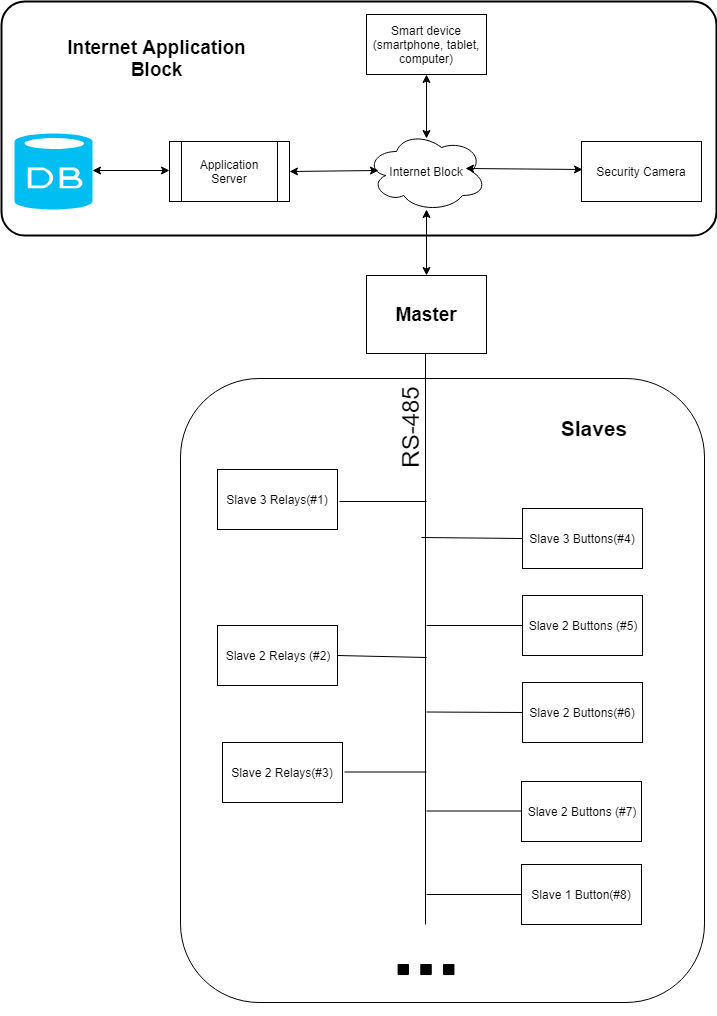
\includegraphics[scale=0.6]{images/blockDiagram.PNG}
        \caption{System Block Diagram}
        \label{fig:blockDiagram}
        \end{center}
    \end{figure}
    Figure~\ref{fig:blockDiagram} refers the overview of the system. From the block diagram, there are three main blocks, namely Master, Slaves and Internet Application block. In this thesis, each main block has different functions and may consists of one to many smaller blocks. Referring to Figure~\ref{fig:blockDiagram}, Master is in the middle, connects Slaves and Internet Application Block; Slaves are the “workers” depend on the Master and the Internet Block helps the User communicate with the system through Master remotely.
    \subsubsection{Master}
    As designed in section \ref{masterDesign}, Master is the circuit integrated with a STM32F4 Discovery Kit, connected via headers instead of being soldered directly on board in order to ensure an effortless replacement if broken. Beside the block of RS-485 module for main communication methodology and ESP-8266 for establishing connection to the Internet, it also has the headers for other modules of connectivity and functions in order to make the Master scalable in the future, namely SIM800A, Bluetooth module HC-05, and Real time module DS3231. However, instead of using an integrated Power block onto Master circuit, it uses a separated Power for Master as mentioned in section \ref{powerForMasterDesign}.

    Based on the basic idea, Master is responsible for receiving the requests from all sources, Slaves or Internet Application block, and distributing the command to the Slave with appropriate function. In addition, Master is also the middleman between Internet Application block with the Slaves, which means it also update the information between Internet application block and Slaves.
    \subsubsection{Slave Relay(s)}
    Slave Relay(s) (Slave \#1, \#2, \#3) consists of number of Relays (varies depends on users’ needs) and one PIC16F628A from Microchip as the MCU, responsible for switching AC devices On or Off based on the distributed command from Master.
    \subsubsection{Slave Button(s)}
    Slave Button(s) (Slave \#4-8) consists of number of Buttons (varies depends on users’ needs) and one PIC16F628A from Microchip as the MCU, responsible for controlling Slave Relay(s) by sending the commands to Master for the distribution to corresponding Slave Relay(s).
    \subsubsection{Internet Application Block}
    Internet Application block consists of smaller blocks with different functions, namely Database, Application Server, Internet connection block, Security Camera and Smart devices. Internet block establish the Internet connection for Master block; Application Server is the combination of back-end and front-end development of Webserver, besides helping users to control the system remotely with ease, the extended features will be explained later in this chapter; Security Camera responsible for recognizing person with Facial Recognition to open the door in order to cut off the steps of accessing the house. In addition, security camera is also integrated with motion detector prototype directly in Application Server.
    \subsection{Communication Methodology and Algorithm}
    In this thesis, data is transmitted from UART of MCU to input of module RS-485 then to the data bus wire to distribute to corresponded components, noted that RS-485 is the physical standard which helps transmitted data travels much further compared to original UART. It needs two wires for data transmitting with module RS-485, but a cable of four wires is chosen for providing power supply of 12VDC and transmitting data at the same time with a single cable. Four wires in a cable with corresponded functions are listed as following.
    \begin{itemize}
    \item 12V: provide 12VDC throughout the system.
    \item A: Signal wire A.
    \item B: Signal wire B.
    \item GND: Common ground throughout the system.
    \end{itemize}

    However, RS-485 is a physical standard instead of an algorithm to distribute data through the whole network of a large number of devices with acceptable performance. Furthermore, in order for the chosen module RS-485 be able to work, its enable pin must be controlled by the MCU, which is set to logic 0 as default is receiving mode and vice versa. After sometimes reading books, the author suggested two algorithms for this thesis.
    \subsubsection{Ask/Request sequentially}
    \begin{itemize}
    \item \textbf{Master}: Master responsible for asking sequentially every connected Slaves in the system. After asking the Slaves for if they need to work, Master will delay for a small amount of time to wait for the response from Slaves. If the time is passed and asked Slave does not request to work, Master will pass that Slave and move on the next Slave. If a Slave Button is being asked but also receive the external signal, it can interrupt the process by sending a response to Master requesting to work, then that request will be prior to be sent to corresponded Slave Device. Now it ends the loop and start a new one. Period of time to ask the Slaves must be in milliseconds in order to complete the loop for every Slaves in the system.
    \item \textbf{Slave Button}: Slave Button has to wait for Master to ask and response. It is always stay in receiving mode (which has enable pin logic at 0 – LOW). When Slave Button is asked or an external signal comes in, it pulls enable pin to logic 1-HIGH to enter transmitting mode and response when Master asks.
    \item \textbf{SLave Device}: Enable pin of RS-485 of Slave Device is always in LOW status, which means receiving data mode. When Master ask or there is data transmitted from Slave Button, Slave Device will check if it is corresponded with its functions, if yes Slave Device will work as defined function.
    \end{itemize}
    
    With this algorithm, the asking loops will run continuously, and it should prevent two signal collide with one and another because the Slave only answers Master when Master asks. However, transmitted data will be difficult to be managed because of two reasons, waiting time and management. After a request is sent from Master, it takes some time for Master to wait for the response from Slave and pull enable pin of RS-485 to LOW. Besides, it takes times again to pull enable pin up to logic HIGH to distribute the response if available. This process is getting longer with the increment of the number of Slaves, which cause the transmission between Slaves become slower with a large number of Slaves. Furthermore, transmitting data continuously will consume loads of bandwidth leads to resource waste and cause errors dues to noise or inaccurate process from Slaves because of data is transmitted continuously leads to false data or worse is lose data. Thus, the author chose a different method to transmit data through the network based on CSMA/CD protocol.
    



